\def \kaflanr {10}
\lecture[\kaflanr]{\kaflanr. Útgildi}{lecture-text}
\date{4.~febrúar 2015}
\newcounter{mycount}
\refstepcounter{mycount}

\begin{document}

\begin{frame}
	\maketitle
\end{frame}

%x


\begin{frame}{Útgildi} 

\begin {block}{Skilgreining \kaflanr.\arabic{mycount}}\stepcounter{mycount}
 Látum $f$ vera fall af tveim breytum
skilgreint á mengi ${\cal D}(f)$.  

\medskip
Sagt er að $f$ hafi {\em \color{red} staðbundið
  lággildi} (e.~local minimum) í punkti $(a,b)$ ef til er tala $r>0$ þannig að 
$f(a,b)\leq f(x,y)$ fyrir alla punkta $(x,y)\in B_r(a,b)\cap{\cal
  D}(f)$.

\medskip
Sagt er að $f$ hafi {\em \color{red} staðbundið
  hágildi}  (e.~local maximum) í punkti $(a,b)$ ef til er tala $r>0$ þannig að 
$f(a,b)\geq f(x,y)$ fyrir alla punkta $(x,y)\in B_r(a,b)\cap{\cal
  D}(f)$.

\medskip
Í þeim punktum þar sem $f$ tekur annað hvort staðbundið lággildi eða
staðbundið hágildi er sagt að $f$ hafi {\em \color{red} staðbundið útgildi}
(e.~local extreme). 


\medskip
Ef $f(a,b)\leq f(x,y)$ fyrir alla punkta $(x,y)\in {\cal D}(f)$ þá er
sagt að $f$ taki {\em \color{red} lægsta gildi} í $(a,b)$ (e.~global minimum).
Ef $f(a,b)\geq f(x,y)$ fyrir alla punkta $(x,y)\in {\cal D}(f)$ þá er
sagt að $f$ taki {\em \color{red} hæsta gildi} í $(a,b)$ (e.~global maximum).

\end{block}

\end{frame}
%x


\begin{frame}{Staðbundið útgildi} 

\begin {block}{Upprifjun \kaflanr.\arabic{mycount}}\stepcounter{mycount}
   Látum $f$ vera fall af einni breytu
skilgreint á mengi ${\cal D}(f)\subseteq \R$.  Ef fallið $f$ hefur
staðbundið útgildi í punkti $a$ þá gildir eitt af þrennu um $a$:

\begin {enumerate}
 \item $f'(a)=0$. \qquad (punkturinn $a$ kallast {\em \color{red} stöðupunktur} $f$).
 \item Afleiðan $f'(a)$ er ekki skilgreind.
 \item   Punkturinn $a$ er jaðarpunktur ${\cal D}(f)$.
\end {enumerate}

\end{block}

\end{frame}
%x


\begin{frame}{Staðbundið útgildi} 

\begin {block}{Setning \kaflanr.\arabic{mycount}}\stepcounter{mycount}
 Látum $f$ vera fall af tveim breytum
skilgreint á mengi ${\cal D}(f)\subseteq \R^2$.  Ef fallið $f$ hefur
staðbundið útgildi í punkti $(a,b)$ þá gildir eitt af þrennu um $a$
\begin {enumerate}
 \item  $\nabla f(a,b)=\ov$. \qquad (punkturinn $(a,b)$ kallast {\em \color{red}
     stöðupunktur} $f$) 
\item Stigullinn $\nabla f(a,b)$ er ekki skilgreindur.
\item Punkturinn $(a,b)$ er jaðarpunktur ${\cal D}(f)$.
\end {enumerate}

\end{block}

\end{frame}
%x

\begin {frame}
  Dæmi: Föll skilgreind á svæðinu $-0.5 \leq x \leq 0.5$,  $-0.5 \leq y \leq 0.5$. Hvar eru staðbundin hágildi?
  \begin{figure}[!h]
        \centering
        \begin{minipage}{.5\textwidth}
            \centering
            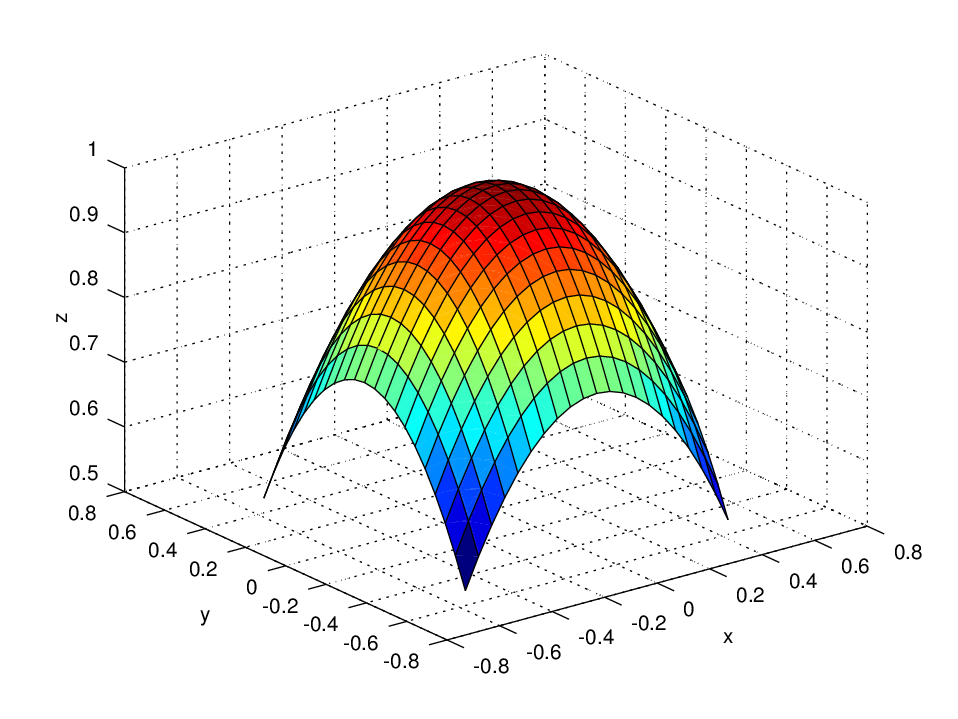
\includegraphics[width=.8\linewidth]{peak_smooth.png}
            \caption*{$z = f(x,y) = 1-x^2-y^2$.}
        \end{minipage}%
        \begin{minipage}{.5\textwidth}
            \centering
            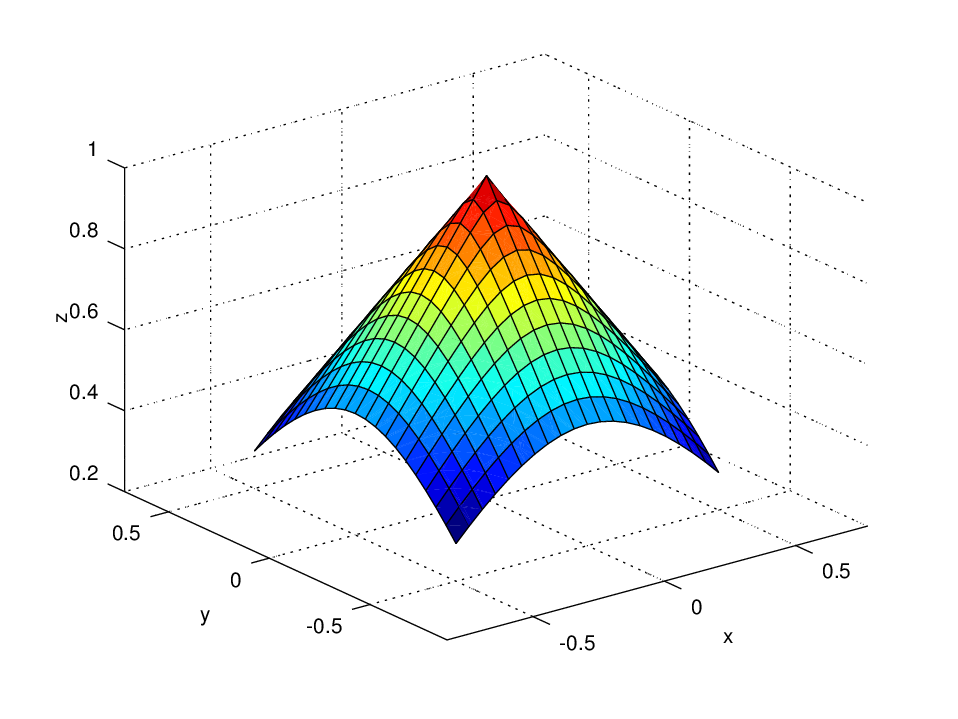
\includegraphics[width=.8\linewidth]{peak.png}
            \caption*{$z = f(x,y) = 1-\sqrt{x^2+y^2}$.}
        \end{minipage}
        \begin{minipage}{.5\textwidth}
            \centering
            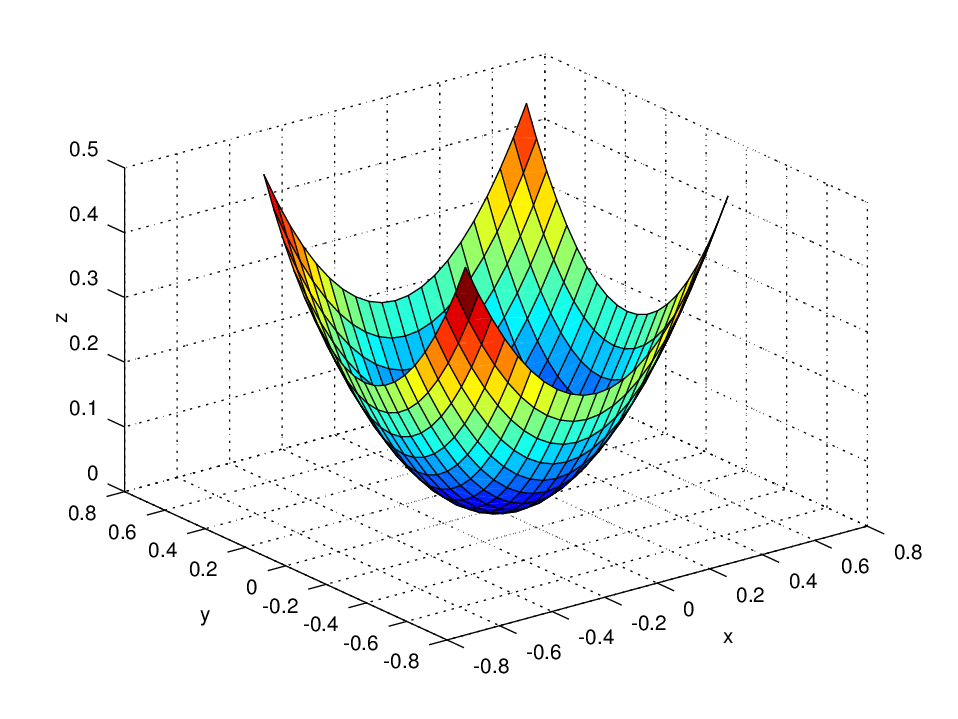
\includegraphics[width=.8\linewidth]{max_bound.png}
            \caption*{$z= f(x,y) = x^2+y^2$.}
        \end{minipage}
    \end{figure}
\end {frame}




\begin{frame}{Tilvist útgilda} 

\begin {block}{Setning \kaflanr.\arabic{mycount}}\stepcounter{mycount}
Látum $f$ vera samfellt fall af tveim breytum
skilgreint á lokuðu og takmörkuðu mengi ${\cal D}(f)$.  Fallið $f$
  tekur þá bæði hæsta og lægsta gildi. 

\end{block}

\end{frame}
%x


\begin{frame}{Söðulpunktur} 

\begin {block}{Skilgreining \kaflanr.\arabic{mycount}}\stepcounter{mycount}
 Punktur $(x,y)\in  {\cal D}(f)$ sem er ekki
jaðarpunktur kallast {\em \color{red} söðulpunktur} ef $\nabla f(x,y)=\ov$ en $f$
hefur ekki staðbundið útgildi í $(x,y)$.
\end{block}

\end{frame}
%x

\begin {frame}
Dæmi um föll með söðulpunkta.
   \begin{figure}[!h]
        \centering
        \begin{minipage}{.5\textwidth}
            \centering
            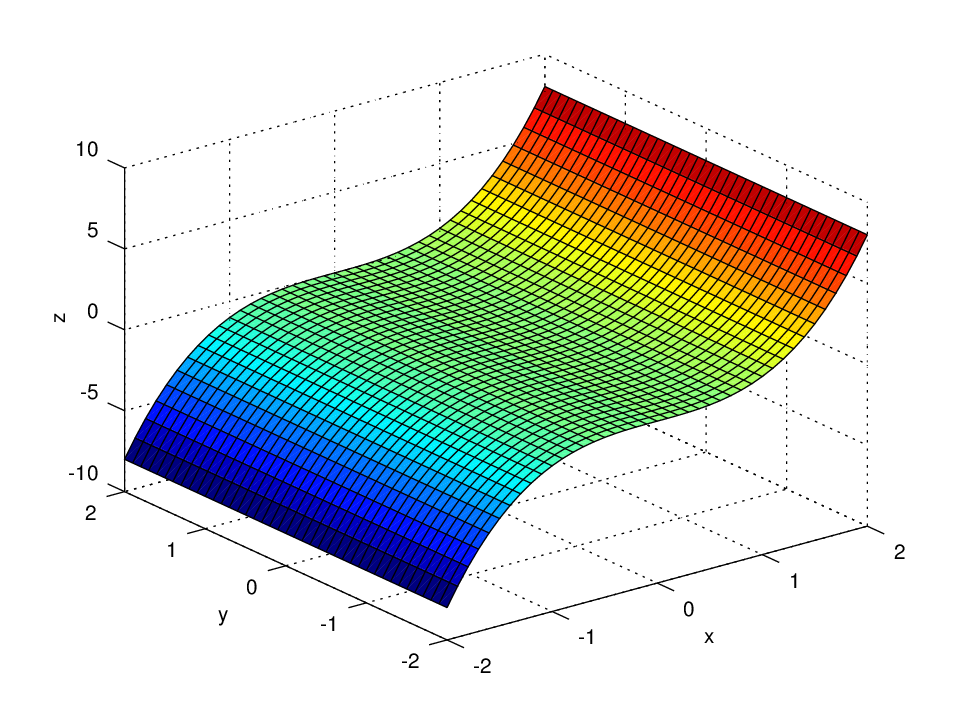
\includegraphics[width=.9\linewidth]{sodull1.png}
            \caption*{$z = f(x,y) = x^3$.}
        \end{minipage}%
        \begin{minipage}{.5\textwidth}
            \centering
            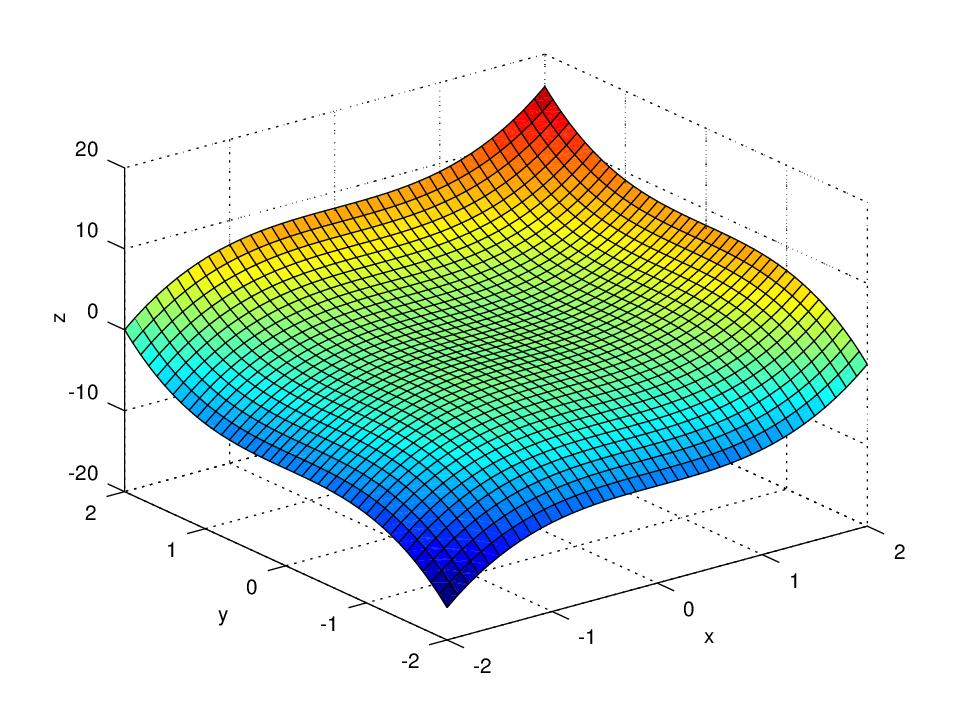
\includegraphics[width=.9\linewidth]{sodull2.png}
            \caption*{$z = f(x,y) = x^3+y^3$.}
        \end{minipage}
        
    \end{figure}
\end {frame}


\begin{frame}{Staðbundið útgildi} 

\begin {block}{Upprifjun \kaflanr.\arabic{mycount}}\stepcounter{mycount}
 Látum $f$ vera fall af einni breytistærð og
gerum ráð fyrir að $f'$ sé samfellt fall.  Gerum einnig ráð fyrir að
$f'(a)=0$.  Þá gildir: 

\begin {enumerate}
 \item Ef $f''(a)>0$ þá hefur $f$ staðbundið lággildi í $a$.
 \item  Ef $f''(a)<0$ þá hefur $f$ staðbundið hágildi í $a$.
 \item  Ef $f''(a)=0$ þá gæti verið staðbundið lággildi í $A$, það gæti
     verið staðbundið hágildi í $a$ eða það gætu verið beygjuskil í
     $a$, alltsvo. ekkert hægt að segja. 
 \end {enumerate}

\end{block}

\end{frame}
%x


\begin{frame}{Hesse-fylki} 

\begin {block}{Skilgreining \kaflanr.\arabic{mycount}}\stepcounter{mycount}
Látum $f$ vera fall af $n$ breytum $\mathbf{x} = (x_1,x_2,\ldots,x_n)$ og
gerum ráð fyrir að allar 2.~stigs hlutafleiður $f$ séu skilgreindar í
punktinum $\mathbf{x}$.  Skilgreinum  {\em \color{red} Hesse-fylki} $f$ í punktinum
$\mathbf{x}$ sem $n\times n$-fylkið
$${\cal H}(\mathbf{x})=\begin{bmatrix} f_{11}(\mathbf{x})&f_{12}(\mathbf{x}) & \cdots & f_{1n}(\mathbf{x})\\
 f_{21}(\mathbf{x})&f_{22}(\mathbf{x}) & \cdots & f_{2n}(\mathbf{x}) \\
 \vdots & \vdots & \ddots & \vdots & \\
  f_{n1}(\mathbf{x})&f_{n2}(\mathbf{x}) & \cdots & f_{nn}(\mathbf{x})\end{bmatrix}.$$
\end{block}

\end{frame}
%x


\begin{frame}{Ferningsform (sjá kafla 10.7 í Adams)} 

\begin {block}{Upprifjun \kaflanr.\arabic{mycount}}\stepcounter{mycount}
{\em \color{red} Ferningsform} $Q$ af $n$-breytum $x_1,x_2,\ldots, x_n$ er einsleit margliða af stigi 2 gefin með 
\begin {equation*}
Q(\mathbf{x}) = \mathbf{x}^T A \mathbf{x}
\end {equation*}
þar sem $A$ er samhverft $n \times n$ fylki með tölu $a_{ij}$ í sæti $(i,j)$ og $\mathbf{x} = [x_1,x_2,\ldots x_n]^T$.
\end{block}

\end{frame}




\begin{frame}{Ferningsform} 

\begin {block}{Skilgreining \kaflanr.\arabic{mycount}}\stepcounter{mycount}
Ferningsform $Q$ af $n$-breytum er sagt vera
{\em \color{red} jákvætt ákvarðað}\  (e.~positive definite) ef $Q(\xv)>0$ fyrir
alla vigra $\xv\neq \ov$ í $\Rn$.   

\medskip
Sagt að ferningsformið $Q$ sé
{\em \color{red} neikvætt ákvarðað}\  (e.~negative definite) ef $Q(\xv)<0$ fyrir
alla vigra $\xv\neq \ov$ í $\Rn$.   

\medskip
Síðan er sagt að ferningsformið $Q$ sé
{\em  \color{red} óákvarðað}\  (e.~indefinite) ef $Q(\xv)<0$ fyrir
einhvern vigur $\xv$  og $Q(\yv)>0$ fyrir einhvern vigur
$\yv$. 
\end{block}

\end{frame}
%x


\begin{frame}{Ferningsform} 

\begin {block}{Setning \kaflanr.\arabic{mycount}}\stepcounter{mycount}
 Látum $Q$ vera fernings form  af $n$ breytum og
$A$ samhverft $n\times n$ fylki þannig að $Q(\xv)=\xv^TA\xv$ fyrir
alla vigra $\xv$,
\begin {enumerate}
 \item  Ferningsformið er jákvætt ákvarðað ef og aðeins ef öll eigingildi
    $A$ eru jákvæð.
\item Ferningsformið er neikvætt ákvarðað ef og aðeins ef öll eigingildi
    $A$ eru neikvæð.
\item  Ferningsformið er óákvarðað ef og aðeins ef $A$ hefur bæði jákvæð
     og neikvæð eigingildi.	
\end {enumerate}

\end{block}

\end{frame}
%x


\begin{frame}{Staðbundið útgildi} 

\begin {block}{Setning \kaflanr.\arabic{mycount}}\stepcounter{mycount}
 Látum $f$ vera fall af $n$ breytum $\mathbf{x} = (x_1,x_2,\ldots,x_n)$ þannig að allar
1.~og 2.~stigs hlutafleiður $f$ eru samfelldar.  Látum $\mathbf{a}$ vera
innri punkt á skilgreiningarsvæði $f$ og gerum ráð fyrir að $\nabla
f(\mathbf{a})=\ov$.  Þá gildir: Ef ${\cal H}(\mathbf{a})$ er 
\begin {enumerate}
 \item  ...jákvætt ákvarðað þá hefur $f$ staðbundið
     lággildi í $\mathbf{a}$.
\item ...neikvætt ákvarðað þá hefur $f$ staðbundið
     hágildi í $\mathbf{a}$.
\item    ...óákvarðað þá hefur $f$ söðulpunkt í
      $\mathbf{a}$.  
\item ...hvorki jákvætt ákvarðað, neikvætt ákvarðað
      né óákvarðað þá nægja upplýsingarnar sem felast í jöfnunni
      $\nabla f(\mathbf{a})=\ov$ og Hesse-fylkinu ekki til að segja til um
      hvers eðlis stöðupunkturinn $\mathbf{a}$ er.
\end {enumerate}

\end{block}

\end{frame}
%x


\begin{frame}{Staðbundið útgildi}  

\begin {block}{Fylgisetning \kaflanr.\arabic{mycount}}\stepcounter{mycount}
Látum $f$ vera fall af tveim breytum þannig að
1.~og 2.~stigs hlutafleiður $f$ eru samfelldar.  Látum $(a,b)$ vera
innri punkt á skilgreiningarsvæði $f$ og gerum ráð fyrir að $\nabla
f(a,b)=\ov$.  Setjum 
$$A=f_{11}(a,b),\qquad\quad B=f_{12}(a,b)=f_{21}(a,b)\qquad\quad
C=f_{22}(a,b).$$ 
Þá gildir:
\begin {enumerate}
 \item  Ef $B^2-AC<0$ og $A>0$  þá hefur $f$
     staðbundið lággildi í $(a,b)$.
 \item  Ef $B^2-AC<0$ og $A<0$ 
 þá hefur $f$ staðbundið
hágildi í $(a,b)$.
 \item   Ef $B^2-AC>0$ 
þá hefur $f$ söðulpunkt í
      $(a,b)$.  
 \item  Ef $B^2-AC=0$ þá er ekkert hægt að segja.  
\end {enumerate}


\end{block}
 \end {frame}
\begin{frame}{Ferningsform}  

\begin {block}{Regla \kaflanr.\arabic{mycount}}\stepcounter{mycount}
Ef $A$ er samhverft $n \times n$ fylki með tölu $a_{ij}$ í sæti $(i,j)$ og
\begin {equation*}
 D_i = \begin{vmatrix}
        a_{11} & a_{12} & \cdots & a_{1i} \\
        a_{21} & a_{22} & \cdots & a_{2i} \\
        \vdots & \vdots & \ddots & \vdots \\ 
        a_{i1} & a_{i2} & \cdots & a_{ii} 
       \end{vmatrix}
\end {equation*}
þá gildir
\begin {enumerate}
 \item Ef $D_i > 0$ fyrir $1\leq i \leq n$ þá er $A$ jákvætt ákvarðað.
 \item Ef $D_i > 0$ fyrir slétt $i$ í $\{1,2,\ldots,n\}$ og $D_i < 0$ fyrir oddatölu $i$ í $\{1,2,\ldots,n\}$ þá er $A$ neikvætt ákvarðað.
 \item Ef $\det(A) = D_n \neq 0$ en hvorki $1$ né $2$ gilda þá er $A$ óákvarðað. 
 \item Ef $\det(A) = 0$ þá er $A$ hvorki jákvætt né neikvætt ákvarðað en getur verið óákvarðað.
\end {enumerate}


\end{block}
\end{frame}
\end{document}